\chapter{Binary Search Complete Implementation}
\label{binappendix}
The best way to implement the tree data structure is to create a class for the nodes (\textbf{Node}) and a class for the binary tree (\textbf{BinaryTree}). As all the nodes of a binary trees has at most two children, in the class \textbf{Node} is enough to have three attributes: the value of the node, the left, and the right child, in turn of \textbf{Node} type as well. This way of implement tree is very similar to the one used for the \hyperref[linked list]{} linked list (\ref{linkedlist}).

\begin{lstlisting}[firstnumber=1, caption={Class definition for a node and a tree.}]
class Node():

	def __init__(self, value):
		self.value = value
		self.left = None
		self.right = None

class BinaryTree():

	def __init__(self, root):
		self.root = Node(root)
\end{lstlisting}

In this appendix there is a detailed implementation, both recursive and iterative, of all possible ways to perform a tree traversal in the case of \textbf{depth-first search}: pre-order traversal \ref{preorderappendix}, in-order traversal \ref{inorderappendix}, and post-order traversal \ref{postorderappendix}. The convention followed here is to look up first at the left child always, and later look up the right one. The opposite approach is equivalent.

The pseudocode of the iterative implementations is taken from \cite{wikitreestrav}(\href{https://en.wikipedia.org/wiki/Tree_traversal}{Tree traversal, Wikipedia}).

\section{Pre-order Traversal}
\label{preorderappendix}
In the pre-order traversal every new node is first checked as visited, and the left subtree is traversed first, and later the right one. This process is repeated until all the nodes of the tree are visited (\ref{preorder}). 

For implementing the pre-order traversal iteratively a stack (\ref{stack}) is used. The steps are \cite{wikitreestrav}:

\begin{algorithm}[H]
	\DontPrintSemicolon
	\LinesNumbered
  	\SetKwFunction{FIterativePreorder}{Iterative-Preorder}
  	\SetKwFunction{FRecursivePreorder}{Recursive-Preorder}
  	\SetKwProg{Fn}{Function}{:}{}
  	\Fn{\FRecursivePreorder{$node$}}{
		\If{(\normalfont{node == \textbf{null}})}{
			\KwRet
		}
		visit(node)\;
		\FRecursivePreorder{$node.left$}\;
		\FRecursivePreorder{$node.right$}\;
  	}
  	\;
  	\Fn{\FIterativePreorder{$node$}}{
  			s $\leftarrow$ \textbf{empty stack}\;
  			s.push(node)\;
  			\While{(\normalfont{\textbf{not} s.isEmpty()})}{
				node $\leftarrow$ s.pop()\;
				visit(node)\;  			
  				\CommentSty{$/*$ Right child is pushed first so that left is processed first (LIFO) $*/$}\;
  				
  				\If{(\normalfont{node.right $\neq$ \textbf{null}})}{
  					s.push(node.right)\;
  				}
    	    	\If{(\normalfont{node.left $\neq$ \textbf{null}})}{
  					s.push(node.left)\;
  				}
        	}
  	}
\caption{Pre-order pseudocode.}
\end{algorithm}

\begin{lstlisting}[firstnumber=1, caption={Recursive and iterative implementation of pre-order traversal.}]
class BinaryTree():
	...

	def recursive_print_tree(self):
		return self.preorder_recursive_print(tree.root, "")[:-1]
	
	def iterative_print_tree(self):
		return self.preorder_search_iterative(self, tree.root, "")

	def preorder_search_recursive(self, start, find_val):
		if start:
			if start.value == find_val:
				return True
			self.preorder_search_recursive(start.left, find_val)
			self.preorder_search_recursive(start.right, find_val)

	def preorder_search_iterative(self, start, find_val):
		if start == None:
			return None
		visited = []		
		stack = []
		stack.push(start)
		while stack: # Keep cycle until the stack is empty
			node = stack.pop()
			visited.append(node)
			if node.value == find_val:
				return True
			# Right child is pushed first so that the left one is processed first
			if node.right:
				stack.append(node.right)
			if node.left:
				stack.append(node.right)
		return visited

	def preorder_recursive_print(self, start, traversal):
		if start:
			traversal += (str(start.value) + "-")
			traversal = self.preorder_recursive_print(start.left, traversal)
			traversal = self.preorder_recursive_print(start.right,traversal)
		return traversal
\end{lstlisting}

\begin{figure}[H]
	\begin{center}
		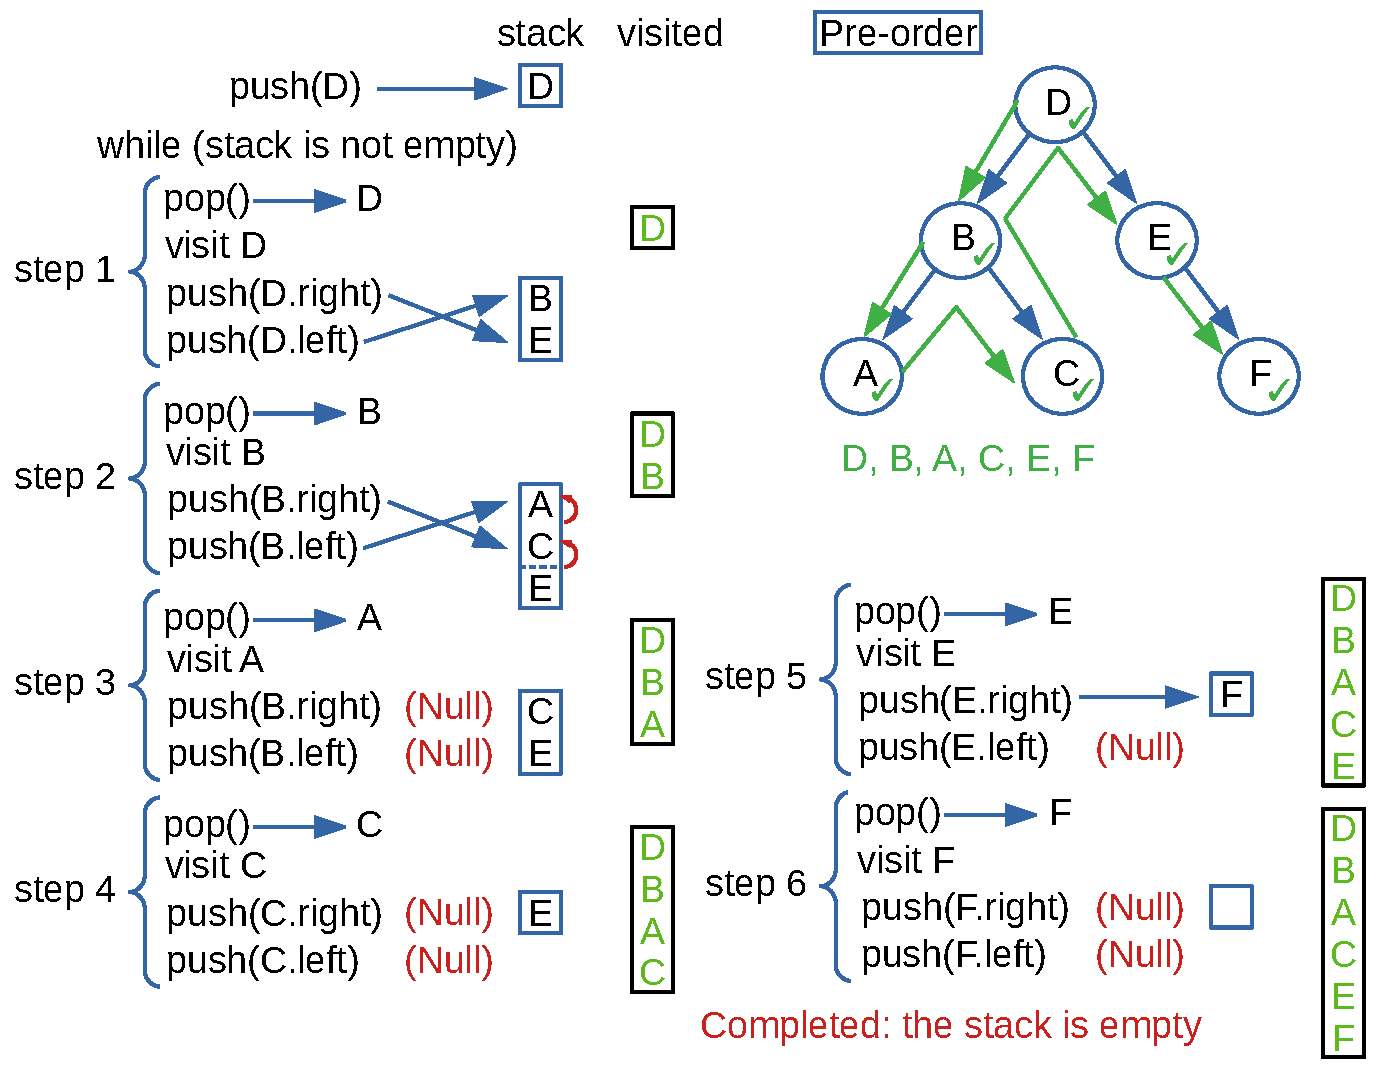
\includegraphics[scale=.6]{chapters/appendix/images/appendixtree/treesappendix_1.pdf}
		\caption[Pre-order iterative example.]{Pre-order iterative example.}
		\label{appendixtrees_1}
	\end{center}
\end{figure}

\begin{figure}[H]
\centering
\begin{tikzpicture}[every node/.style={circle,draw}, node distance=15mm, thick]

\node (na){$a$}
   child{node (nb) {$b$}
             child {node (nd) {$d$}}
             child {node (ne) {$e$}}
        }
   child{node (nc) {$c$}
			child[missing]
			child{node (nf) {$f$}}
		};
\draw ($(na) + (-2, 0.4)$) node[rectangle] {Pre-order};
\draw node[draw=none, rectangle, below=1mm of nd] {a, b, d, e, c, f};
  
  %\fill circle (3pt) node ($(na) + (-0.4,0.2)$) {Here!};
  \fill[color=black] ($(na) + (-0.42,0.2)$) circle (0.1);
  \fill[color=black] ($(nb) + (-0.42,0.2)$) circle (0.1);
  \fill[color=black] ($(nd) + (-0.48,0.0)$) circle (0.1);
  \fill[color=black] ($(ne) + (-0.45,0.0)$) circle (0.1);
  \fill[color=black] ($(nc) + (-0.5,0.15)$) circle (0.1);
  \fill[color=black] ($(nf) + (-0.48,0.0)$) circle (0.1);
  
  \draw[->, >=stealth, BrickRed, rounded corners, dashed, line width=0.7pt]
    ($(na) + (-0.4,0.2)$) --
    ($(nb) + (-0.4,0.2)$) --
    %($(nb) + (-0.44,0.0)$) --
    ($(nd) + (-0.50,0.0)$) --
    ($(nd) + (-0.35,-0.35)$) --
    ($(nd) + (0.0,-0.45)$) --
    ($(nd) + (0.35,-0.35)$) --
    ($(nd) + (0.42,0.0)$) --
    ($(nb) + (0.0,-0.4)$) --
    ($(ne) + (-0.45,0.0)$) --
    ($(ne) + (-0.35,-0.35)$) --
    ($(ne) + (0.0,-0.45)$) --
    ($(ne) + (0.35,-0.35)$) --
    ($(ne) + (0.45,0.0)$) --
    ($(nb) + (0.4,0.0)$) --
    ($(na) + (0.0,-0.4)$) --
    ($(nc) + (-0.5,0.15)$) --
    ($(nf) + (-0.45,0.0)$) --
    ($(nf) + (-0.35,-0.35)$);
    %($(nf) + (0.0,-0.45)$) --
    %($(nf) + (0.35,-0.35)$);
    %($(nf) + (0.48,0.0)$) --
    %($(nc) + (0.42,-0.4)$);
    %($(nc) + (0.36,0.4)$) --
    %($(na) + (0.4,0.2)$);

% Stack 1
\draw ($(na) + (3, 0.4)$) node[draw=none, rectangle, align=left] (stack) {Stack};

\draw[-] ($(stack.west) + (0,-4mm)$) -- ($(stack.west) + (0,-20mm)$);
\draw[-] ($(stack.west) + (10mm,-4mm)$) -- ($(stack.west) + (10mm,-20mm)$);
\draw[-] ($(stack.west) + (0,-20mm)$) -- ($(stack.west) + (10mm,-20mm)$);
\draw ($(stack.south) + (-1mm,-13.5mm)$) node[draw, rectangle, rounded corners, minimum width=0.5cm, minimum height=0.5cm] (a1) {a};
\draw ($(stack.south) + (0,-22mm)$) node[draw, rectangle, minimum width=0.6cm, minimum height=0.6cm] (visited) {\textcolor{ForestGreen}{a}};
\path[->, >=stealth] ($(a1.north west) + (-10mm,3mm)$) edge [bend left=20] node[draw=none, xshift=-6pt, yshift=-7pt] {push} (a1.north west);
\path[->, >=stealth] (a1.north) edge [bend left=20] node[draw=none, xshift=-4pt, yshift=7pt] {pop} ($(a1.north east) + (1mm, 5mm)$);

% Stack 2
\draw ($(stack) + (1, 0)$) node[draw=none, rectangle, align=left] (stack1) {};
\draw[-] ($(stack1.west) + (0,-4mm)$) -- ($(stack1.west) + (0,-20mm)$);
\draw[-] ($(stack1.west) + (10mm,-4mm)$) -- ($(stack1.west) + (10mm,-20mm)$);
\draw[-] ($(stack1.west) + (0,-20mm)$) -- ($(stack1.west) + (10mm,-20mm)$);
\draw ($(stack1.south) + (3.5mm,-15mm)$) node[draw, rectangle, rounded corners, minimum width=0.5cm, minimum height=0.5cm] (c2) {c};
\draw ($(stack1.south) + (3.5mm,-9mm)$) node[draw, rectangle, rounded corners, minimum width=0.5cm, minimum height=0.5cm] (b2) {b};
\draw[->, >=stealth] (a1.east) -- (c2.west);
\draw[->, >=stealth] (a1.east) -- (b2.west);
\draw ($(visited.east) + (10mm,0)$) node[draw, rectangle, minimum width=0.6cm, minimum height=0.6cm] {\textcolor{ForestGreen}{a, b}};

% Stack 3
\draw ($(stack1) + (1.5, 0)$) node[draw=none, rectangle, align=left] (stack2) {};
\draw[-] ($(stack2.west) + (0,-4mm)$) -- ($(stack2.west) + (0,-20mm)$);
\draw[-] ($(stack2.west) + (10mm,-4mm)$) -- ($(stack2.west) + (10mm,-20mm)$);
\draw[-] ($(stack2.west) + (0,-20mm)$) -- ($(stack2.west) + (10mm,-20mm)$);
\draw ($(stack2.south) + (3.5mm,-15mm)$) node[draw, rectangle, rounded corners, minimum width=0.5cm, minimum height=0.5cm] (c3) {c};
\draw ($(stack2.south) + (3.5mm,-9mm)$) node[draw, rectangle, rounded corners, minimum width=0.5cm, minimum height=0.5cm] (e3) {e};
\draw ($(stack2.south) + (3.5mm,-3mm)$) node[draw, rectangle, rounded corners, minimum width=0.5cm, minimum height=0.5cm] (d3) {d};
\draw[->, >=stealth] (b2.east) -- (d3.west);
\draw[->, >=stealth] (b2.east) -- (e3.west);
\draw ($(visited.east) + (25mm,0)$) node[draw, rectangle, minimum width=0.6cm, minimum height=0.6cm] {\textcolor{ForestGreen}{a, b, d}};

% Stack 4
\draw ($(stack2) + (1.5, 0)$) node[draw=none, rectangle, align=left] (stack3) {};
\draw[-] ($(stack3.west) + (0,-4mm)$) -- ($(stack3.west) + (0,-20mm)$);
\draw[-] ($(stack3.west) + (10mm,-4mm)$) -- ($(stack3.west) + (10mm,-20mm)$);
\draw[-] ($(stack3.west) + (0,-20mm)$) -- ($(stack3.west) + (10mm,-20mm)$);
\draw ($(stack3.south) + (3.5mm,-15mm)$) node[draw, rectangle, rounded corners, minimum width=0.5cm, minimum height=0.5cm] (c4) {c};
\draw ($(stack3.south) + (3.5mm,-9mm)$) node[draw, rectangle, rounded corners, minimum width=0.5cm, minimum height=0.5cm] (e4) {e};
\draw ($(visited.east) + (44mm,0)$) node[draw, rectangle, minimum width=0.6cm, minimum height=0.6cm] {\textcolor{ForestGreen}{a, b, d, e}};

% Stack 5
\draw ($(stack) + (-0.45, -2.5)$) node[draw=none, rectangle, align=left] (stack4) {};
\draw[-] ($(stack4.west) + (0,-4mm)$) -- ($(stack4.west) + (0,-20mm)$);
\draw[-] ($(stack4.west) + (10mm,-4mm)$) -- ($(stack4.west) + (10mm,-20mm)$);
\draw[-] ($(stack4.west) + (0,-20mm)$) -- ($(stack4.west) + (10mm,-20mm)$);
\draw ($(stack4.south) + (3.5mm,-15mm)$) node[draw, rectangle, rounded corners, minimum width=0.5cm, minimum height=0.5cm] (c4) {c};
\draw ($(stack4.south) + (1mm,-23mm)$) node[draw, rectangle, minimum width=0.6cm, minimum height=0.6cm] {\textcolor{ForestGreen}{a, b, d, e, c}};

% Stack 6
\draw ($(stack4) + (1.45, 0)$) node[draw=none, rectangle, align=left] (stack5) {};
\draw[-] ($(stack5.west) + (0,-4mm)$) -- ($(stack5.west) + (0,-20mm)$);
\draw[-] ($(stack5.west) + (10mm,-4mm)$) -- ($(stack5.west) + (10mm,-20mm)$);
\draw[-] ($(stack5.west) + (0,-20mm)$) -- ($(stack5.west) + (10mm,-20mm)$);
\draw ($(stack5.south) + (3.5mm,-15mm)$) node[draw, rectangle, rounded corners, minimum width=0.5cm, minimum height=0.5cm] (f5) {f};
\draw ($(stack5.south) + (10mm,-23mm)$) node[draw, rectangle, minimum width=0.6cm, minimum height=0.6cm] {\textcolor{ForestGreen}{a, b, d, e, c, f}};

% Stack 7
\draw ($(stack5) + (1.5, 0)$) node[draw=none, rectangle, align=left] (stack6) {};
\draw[-] ($(stack6.west) + (0,-4mm)$) -- ($(stack6.west) + (0,-20mm)$);
\draw[-] ($(stack6.west) + (10mm,-4mm)$) -- ($(stack6.west) + (10mm,-20mm)$);
\draw[-] ($(stack6.west) + (0,-20mm)$) -- ($(stack6.west) + (10mm,-20mm)$);
\draw ($(stack6.east) + (20mm,-10mm)$) node[draw=none, rectangle, minimum width=0.6cm, minimum height=0.6cm] {\textcolor{BrickRed}{Stack empty}};

\end{tikzpicture}

\caption[Pre-order iterative example.]{Pre-order iterative example.}
\label{appendixtrees_1}
\end{figure}

\section{In-order Traversal}
\label{inorderappendix}
In the in-order traversal the first node to be checked is the first leaf of the left subtree. The second one is the parent of the first checked node, and then the right subtree is checked repeating the previous process. All this process is repeated until all the nodes are visited or the value is found \ref{inorder}. 

For implementing the in-order traversal iteratively a stack is used. The steps are \cite{wikitreestrav}:

\begin{algorithm}[H]
	\DontPrintSemicolon
	\LinesNumbered
  	\SetKwFunction{FIterativeInorder}{Iterative-Inorder}
  	\SetKwFunction{FRecursiveInorder}{Recursive-Inorder}
  	\SetKwProg{Fn}{Function}{:}{}
  	\Fn{\FRecursiveInorder{$node$}}{
		\If{(\normalfont{node == \textbf{null}})}{
			\KwRet
		}
		\FRecursiveInorder{$node.left$}\;
		visit(node)\;
		\FRecursiveInorder{$node.right$}\;
  	}
  	\;
  	\Fn{\FIterativeInorder{$node$}}{
  			s $\leftarrow$ \textbf{empty stack}\;
  			\While{(\normalfont{\textbf{not} s.isEmpty() \textbf{or} node $\neq$ \textbf{null}})}{
  				\If{(\normalfont{node $\neq$ \textbf{null}})}{
  					s.push(node)\;
  					node $\leftarrow$ node.left\;
  				}
    	    	\Else{
    	    		node $\leftarrow$ s.pop()\;
    	    		visit(node)\;
    	    		node $\leftarrow$ node.right\;
    	    	}
        	}
  	}
\caption{In-order pseudocode.}
\end{algorithm}

\begin{lstlisting}[firstnumber=1, caption={Recursive and iterative implementation of in-order traversal.}]
class BinaryTree():
	...

	def recursive_print_tree(self):
		return self.inorder_recursive_print(tree.root, "")[:-1]
	
	def iterative_print_tree(self):
		return self.inorder_search_iterative(self, tree.root, "")

	def inorder_search_recursive(self, start, find_val):
		if start:
			self.inorder_search_recursive(start.left, find_val)
			if start.value == find_val:
				return True
			self.inorder_search_recursive(start.right, find_val)

	def inorder_search_iterative(self, start, find_val):
		if start == None:
			return None
		stack = []
		stack.append(start)
		current = start
		visited = []
		while stack or current != None:
			if current != None:
				stack.append(current)
				current = current.left
			else:
				current = stack.pop()
				if current.value == find_val:
					return True
				visited.append(current)
				current = current.right
		return visited		
		
	def inorder_recursive_print(self, start, traversal):
		if start:
			traversal = self.inorder_recursive_print(start.left, traversal)
			traversal += (str(start.value) + "-")
			traversal = self.inorder_recursive_print(start.right,traversal)
		return traversal
\end{lstlisting}

\begin{figure}[H]
	\begin{center}
		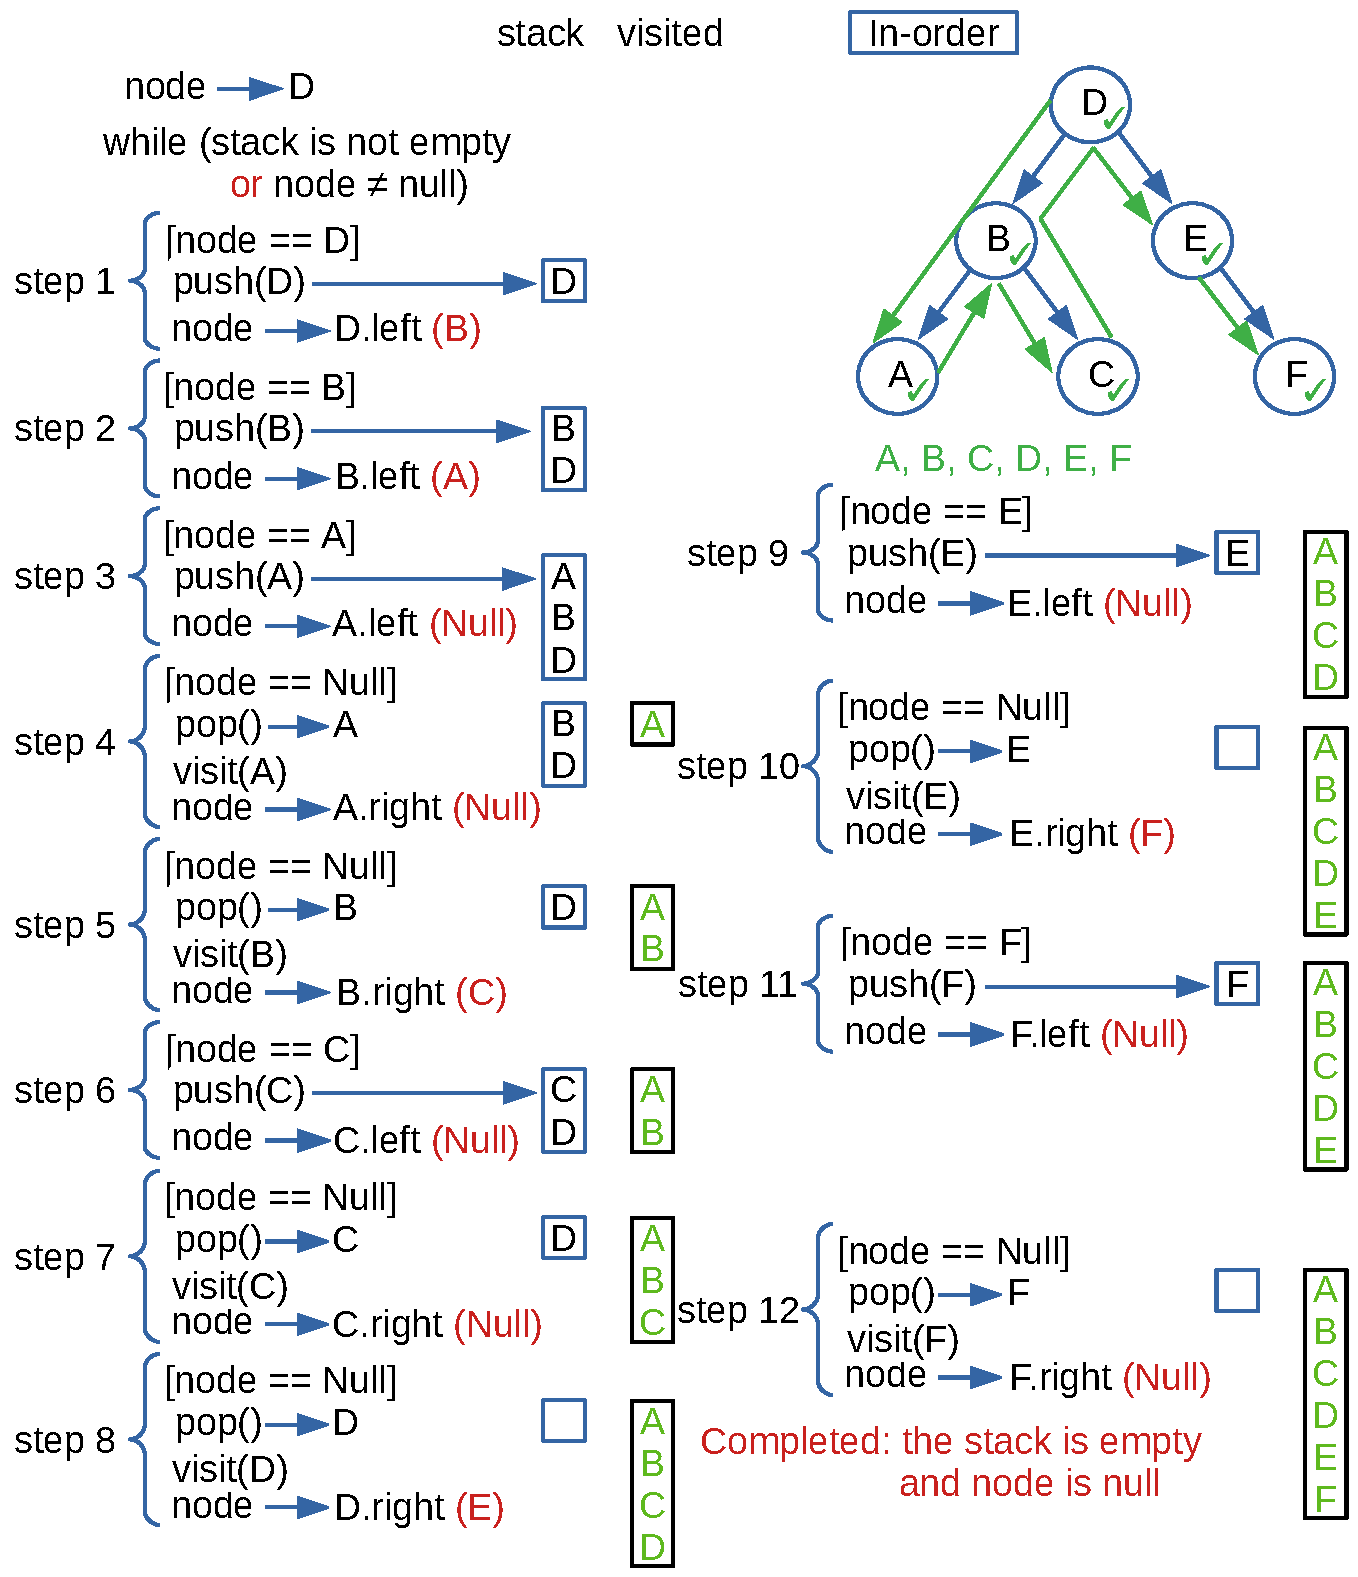
\includegraphics[scale=.6]{chapters/appendix/images/appendixtree/treesappendix_2.pdf}
		\caption[In-order iterative example.]{In-order iterative example.}
		\label{appendixtrees_2}
	\end{center}
\end{figure}

\begin{figure}[H]
\centering
\begin{tikzpicture}[every node/.style={circle,draw}, node distance=15mm, thick]

\node (na){$a$}
   child{node (nb) {$b$}
             child {node (nd) {$d$}}
             child {node (ne) {$e$}}
        }
   child{node (nc) {$c$}
			child[missing]
			child{node (nf) {$f$}}
		};
\draw ($(na) + (-2, 0.4)$) node[rectangle] {In-order};
\draw node[draw=none, rectangle, right=5mm of na] {d, b, e, a, c, f};
  
  %\fill circle (3pt) node ($(na) + (-0.4,0.2)$) {Here!};
  \fill[color=black] ($(nd) + (-0.48,0.0)$) circle (0.1);
  \fill[color=black] ($(nb) + (0.0,-0.5)$) circle (0.1);
  \fill[color=black] ($(ne) + (-0.45,0.0)$) circle (0.1);
  \fill[color=black] ($(na) + (0.0,-0.5)$) circle (0.1);
  \fill[color=black] ($(nf) + (-0.48,0.0)$) circle (0.1);
  \fill[color=black] ($(nc) + (-0.5,0.15)$) circle (0.1);
  
  \draw[->, >=stealth, BrickRed, rounded corners, dashed, line width=0.7pt]
    ($(na) + (-0.4,0.2)$) --
    ($(nb) + (-0.4,0.2)$) --
    %($(nb) + (-0.44,0.0)$) --
    ($(nd) + (-0.50,0.0)$) --
    ($(nd) + (-0.35,-0.35)$) --
    ($(nd) + (0.0,-0.45)$) --
    ($(nd) + (0.35,-0.35)$) --
    ($(nd) + (0.42,0.0)$) --
    ($(nb) + (0.0,-0.4)$) --
    ($(ne) + (-0.45,0.0)$) --
    ($(ne) + (-0.35,-0.35)$) --
    ($(ne) + (0.0,-0.45)$) --
    ($(ne) + (0.35,-0.35)$) --
    ($(ne) + (0.45,0.0)$) --
    ($(nb) + (0.4,0.0)$) --
    ($(na) + (0.0,-0.4)$) --
    ($(nc) + (-0.5,0.15)$) --
    ($(nf) + (-0.45,0.0)$) --
    ($(nf) + (-0.35,-0.35)$);
    %($(nf) + (0.0,-0.45)$);
    %($(nf) + (0.35,-0.35)$);
    %($(nf) + (0.48,0.0)$);
    %($(nc) + (0.64,-0.4)$) --
    %($(nc) + (0.30,0.4)$);
    %($(na) + (0.4,0.2)$);

\end{tikzpicture}

\begin{tabular}{ l|c|c|c|c|c|c } 
 Step & Node & push & pop & Stack & New Node & Visit \\
 \hline
 1  & a & a & & a & a.left(\textcolor{BrickRed}{b}) & \\
 
 2  & b & b & & b,a & b.left(\textcolor{BrickRed}{d}) & \\
 
 3  & d & d & & d,b,a & d.left(\textcolor{BrickRed}{null}) & \\
 
 4  & null & & d & b,a & d.right(\textcolor{BrickRed}{null}) & \textcolor{ForestGreen}{d} \\
 
 5  & null & & b & a & b.right(\textcolor{BrickRed}{e}) & \textcolor{ForestGreen}{b} \\
 
 6  & e & e &  & e,a & e.left(\textcolor{BrickRed}{null}) & \\
 
 7  & null & & e & a & e.right(\textcolor{BrickRed}{null}) & \textcolor{ForestGreen}{e} \\
 
 8  & null & & a & & a.right(\textcolor{BrickRed}{c}) & \textcolor{ForestGreen}{a} \\
 
 9  & c & c &  & c & c.left(\textcolor{BrickRed}{null}) & \\
 
 10 & null & & c &  & c.right(\textcolor{BrickRed}{f}) & \textcolor{ForestGreen}{c} \\
 
 11 & f & f &  & f & f.left(\textcolor{BrickRed}{null}) & \\
 
 12 & null & & f & & f.right(\textcolor{BrickRed}{null}) & \textcolor{ForestGreen}{f} \\

\textcolor{BrickRed}{stop} & \textcolor{BrickRed}{null} &  & & \textcolor{BrickRed}{empty} & & \\
\end{tabular}
\caption[In-order iterative example.]{In-order iterative example.}
\label{appendixtrees_2}
\end{figure}

\section{Post-order Traversal}
\label{postorderappendix}
In the post-order traversal the first node to be checked is the first leaf of the left subtree. The second node is the right node of the parent of the first checked node. Once checked the right side of the subtree also the parent is checked and the process is repeated until all the node are visited or the value is found \ref{postorder}. 

Also in this case for implementing the post-order traversal iteratively a stack is used. The steps are \cite{wikitreestrav}:

\begin{algorithm}[H]
	\DontPrintSemicolon
	\LinesNumbered
  	\SetKwFunction{FIterativePostorder}{Iterative-Postorder}
  	\SetKwFunction{FRecursivePostorder}{Recursive-Postorder}
  	\SetKwProg{Fn}{Function}{:}{}
  	\Fn{\FRecursivePostorder{$node$}}{
		\If{(\normalfont{node == \textbf{null}})}{
			\KwRet
		}
		\FRecursivePostorder{$node.left$}\;
		\FRecursivePostorder{$node.right$}\;
		visit(node)\;
  	}
  	\;
  	\Fn{\FIterativePostorder{$node$}}{
  			s $\leftarrow$ \textbf{empty stack}\;
  			lastNodeVisited $\leftarrow$ \textbf{null}\;
  			\While{(\normalfont{\textbf{not} s.isEmpty() \textbf{or} node $\neq$ \textbf{null}})}{
  				\If{(\normalfont{node $\neq$ \textbf{null}})}{
  					s.push(node)\;
  					node $\leftarrow$ node.left\;
  				}
    	    	\Else{
    	    		peekNode $\leftarrow$ s.peek()\;
    	    		\CommentSty{$/*$ If right child exists and traversing node from left child, then move right $/*$}\;
    	    		
    	    		\If{(\normalfont{peekNode.right $\neq$ \textbf{null} \textbf{and} lastNodeVisited $\neq$ peekNode.right})}{
    	    			node $\leftarrow$ peekNode.right\;
    	    		}
    	    		\Else{
    	    			visit(peekNode)\;
    	    			lastVisitedNode $\leftarrow$ s.pop()\;
    	    		}
    	    	}
        	}
  	}
\caption{Post-order pseudocode.}
\end{algorithm}

\begin{lstlisting}[firstnumber=1, caption={Recursive and iterative implementation of post-order traversal.}]
class BinaryTree():
	...

	def recursive_print_tree(self):
		return self.postorder_recursive_print(tree.root, "")[:-1]
	
	def iterative_print_tree(self):
		return self.postorder_search_iterative(tree.root, "")

	def postorder_search_recursive(self, start, find_val):
		if start:
			self.postorder_search_recursive(start.left, find_val)
			self.postorder_search_recursive(start.right, find_val)
			if start.value == find_val:
				return True

	def postorder_search_iterative(self, start, find_val):
		if start == None:
			return None
		stack = []
		stack.push(start)
		last_visited_node = None
		visited = []
		current = start
		while stack or current != None:
			if current != None:
				s.push(current)
				current = current.left
			else:
				# Take the last element of the stack
				peeked_node = stack[-1]
				# If right child exists and traversing node from left child, then move right
				if (peeked_node.right != null and last_visited_node != peeked_node.right):
					current = peeked_node.right
				else:
					if peeked_node.value == find_val:
						return True
					visited.append(peeked_node)
					last_visited_node = stack.pop()
		return visited

	def postorder_recursive_print(self, start, traversal):
		if start:
			traversal = self.postorder_recursive_print(start.left, traversal)
			traversal = self.postorder_recursive_print(start.right,traversal)
			traversal += (str(start.value) + "-")
		return traversal
\end{lstlisting}

\begin{figure}[H]
	\begin{center}
		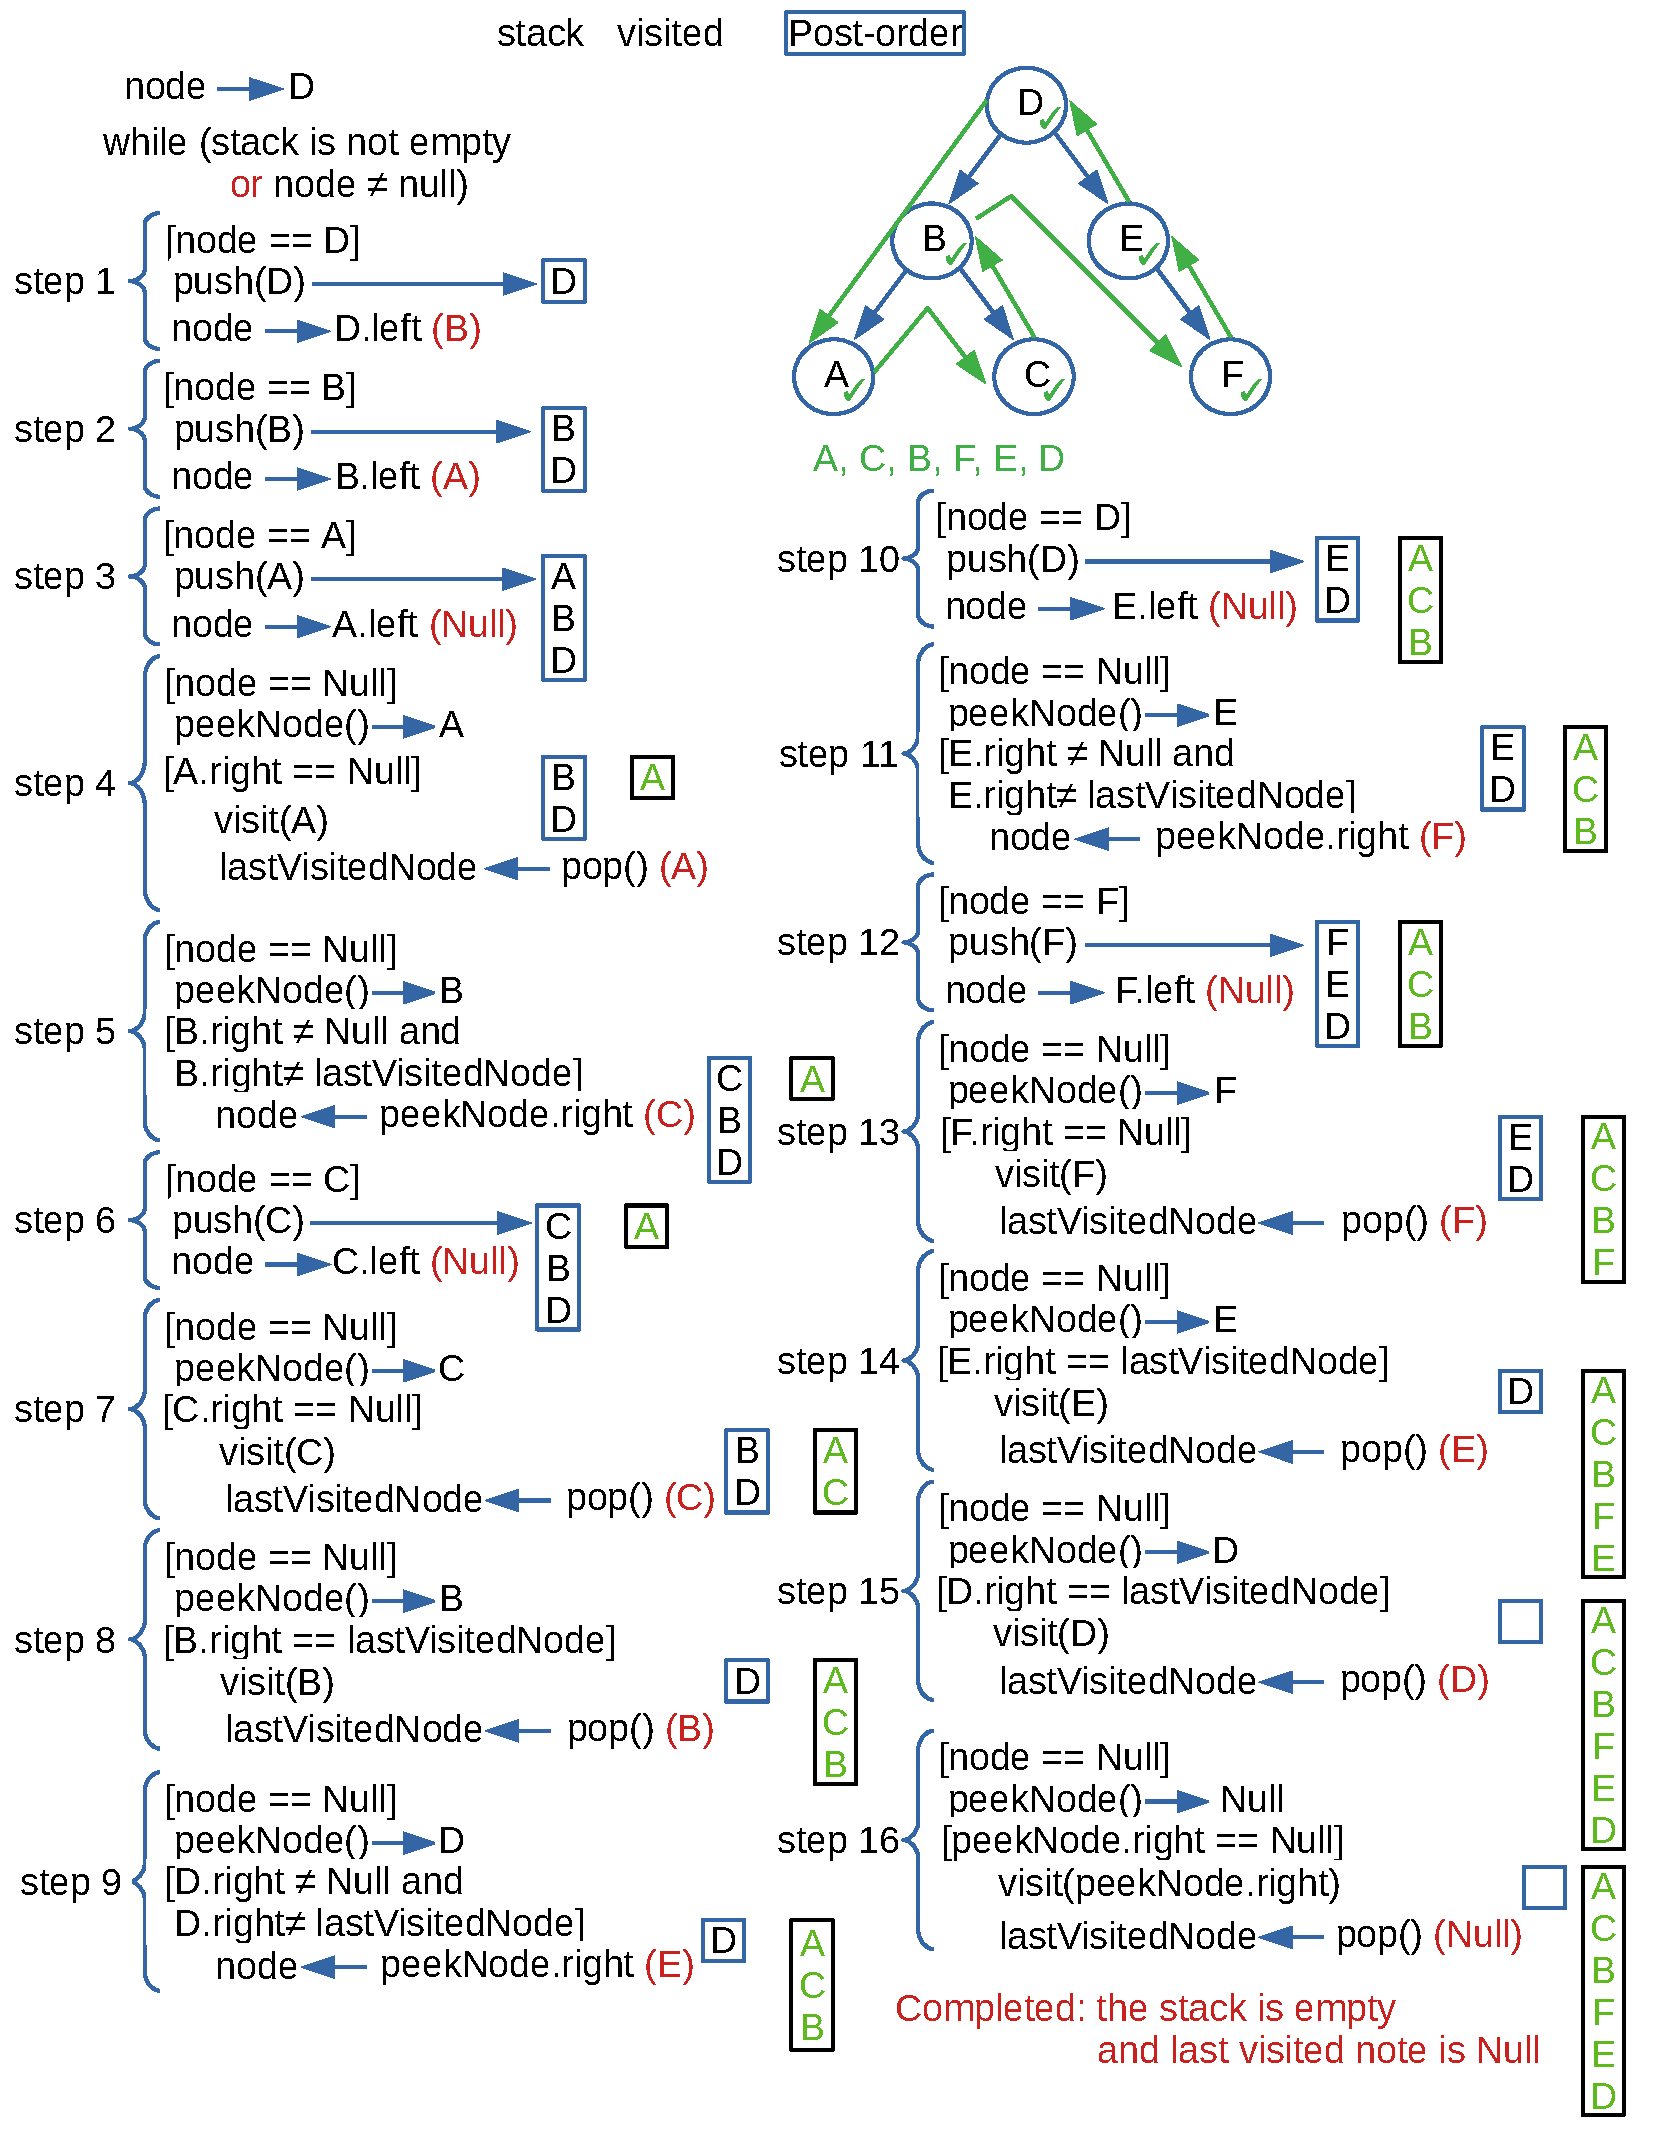
\includegraphics[scale=.6]{chapters/appendix/images/appendixtree/treesappendix_3.pdf}
		\caption[Post-order iterative example.]{Post-order iterative example.}
		\label{appendixtrees_3}
	\end{center}
\end{figure}

\begin{figure}[H]
\centering
\begin{tikzpicture}[every node/.style={circle,draw}, node distance=15mm, thick]

\node (na){$a$}
   child{node (nb) {$b$}
             child {node (nd) {$d$}}
             child {node (ne) {$e$}}
        }
   child{node (nc) {$c$}
			child[missing]
			child{node (nf) {$f$}}
		};
\draw ($(na) + (-2, 0.4)$) node[rectangle] {Post-order};
\draw node[draw=none, rectangle, right=5mm of na] {d, e, b, f, c, a};
  
  %\fill circle (3pt) node ($(na) + (-0.4,0.2)$) {Here!};
  \fill[color=black] ($(nd) + (-0.48,0.0)$) circle (0.1);
  \fill[color=black] ($(ne) + (-0.45,0.0)$) circle (0.1);
  \fill[color=black] ($(nb) + (0.45,0.0)$) circle (0.1);
  \fill[color=black] ($(nf) + (-0.48,0.0)$) circle (0.1);
  \fill[color=black] ($(nc) + (0.44,0.0)$) circle (0.1);
  \fill[color=black] ($(na) + (0.5,0.0)$) circle (0.1);
  
  \draw[->, >=stealth, BrickRed, rounded corners, dashed, line width=0.7pt]
    ($(na) + (-0.4,0.2)$) --
    ($(nb) + (-0.4,0.2)$) --
    %($(nb) + (-0.44,0.0)$) --
    ($(nd) + (-0.50,0.0)$) --
    ($(nd) + (-0.35,-0.35)$) --
    ($(nd) + (0.0,-0.45)$) --
    ($(nd) + (0.35,-0.35)$) --
    ($(nd) + (0.42,0.0)$) --
    ($(nb) + (0.0,-0.4)$) --
    ($(ne) + (-0.45,0.0)$) --
    ($(ne) + (-0.35,-0.35)$) --
    ($(ne) + (0.0,-0.45)$) --
    ($(ne) + (0.35,-0.35)$) --
    ($(ne) + (0.45,0.0)$) --
    ($(nb) + (0.4,0.0)$) --
    ($(na) + (0.0,-0.4)$) --
    ($(nc) + (-0.5,0.15)$) --
    ($(nf) + (-0.45,0.0)$) --
    ($(nf) + (-0.35,-0.35)$) --
    ($(nf) + (0.0,-0.45)$) --
    ($(nf) + (0.35,-0.35)$) --
    ($(nf) + (0.48,0.0)$) --
    ($(nc) + (0.64,-0.4)$) --
    ($(nc) + (0.30,0.4)$) --
    ($(na) + (0.3,0.4)$);
\end{tikzpicture}
\begin{tabular}{ l|c|c|c|c|c|c|c|c} 
 Step & Node & New Node & Last Visited & peek & push & pop & Stack & Visit \\
 \hline
1 & a & a.left (\textcolor{BrickRed}{b}) & & & a & & a & \\
 
2 & b & b.left (\textcolor{BrickRed}{d}) & & & b & & b, a & \\
 
3 & d & d.left (\textcolor{BrickRed}{null}) & & & d & & d, b, a & \\
 
4 & \textcolor{BrickRed}{null} & d.right (\textcolor{BrickRed}{null}) & d & d & & d & b, a & \textcolor{ForestGreen}{d}\\
 
5 & \textcolor{BrickRed}{null} & b.right (\textcolor{BrickRed}{e}) & d & b & & & b, a & \\
 
6 & e & e.left (\textcolor{BrickRed}{null}) & d & & e & & e, b, a & \\
 
7 & \textcolor{BrickRed}{null} & e.right (\textcolor{BrickRed}{null}) & e & e & & e & b, a & \textcolor{ForestGreen}{e} \\
 
8 & \textcolor{BrickRed}{null} & b.right (\textcolor{BrickRed}{e}) == last visited & e & b & & b & a & \textcolor{ForestGreen}{b} \\
 
9 & \textcolor{BrickRed}{null} & a.right (\textcolor{BrickRed}{c}) $\neq$ last visited & e & a & & & a & \\
 
10 & c & c.left (\textcolor{BrickRed}{null}) & e &  & c &  & c,a & \\
  
11 & \textcolor{BrickRed}{null} & c.right (\textcolor{BrickRed}{f}) $\neq$ last visited & e & c & & & c,a & \\

12 & f & f.left (\textcolor{BrickRed}{null}) & e & & f & & f,c,a & \\

13 & \textcolor{BrickRed}{null} & f.right (\textcolor{BrickRed}{null}) & f & f & & f & c,a & \textcolor{ForestGreen}{f} \\

14 & \textcolor{BrickRed}{null} & c.right (\textcolor{BrickRed}{f}) == last visited & f & c & & c & a & \textcolor{ForestGreen}{c} \\

15 & \textcolor{BrickRed}{null} & a.right (\textcolor{BrickRed}{c}) == last visited & a & a & & a &  & \textcolor{ForestGreen}{a} \\

16 & \textcolor{BrickRed}{null} & \textcolor{BrickRed}{null} & \textcolor{BrickRed}{null} & \textcolor{BrickRed}{null} & \textcolor{BrickRed}{null} &  & \textcolor{BrickRed}{empty} & \\

\textcolor{BrickRed}{stop} & & &  & & &  &  &  \\
 
\end{tabular}
\caption[Post-order search.]{Post-order search.}
\label{trees_7}
\end{figure}

\section{Breadth-first search Implementation}
In the case of the \textbf{breadth-first search} (Chapter \ref{chp:trees}) the implementation uses a queue (Section \ref{queue}) instead of a stack. Also here the convention is to check the left node first and later the right ones. The pesudocode is adapted from the general case of the breadth-first search taken from here \cite{wikibreadthfirst} (\href{https://en.wikipedia.org/wiki/Breadth-first_search}{Breadth-first search, Wikipedia}).

\begin{algorithm}[H]
	\DontPrintSemicolon
	\LinesNumbered
  	\SetKwFunction{FBreadthFirstSearch}{Breadth-first-search}
  	\SetKwProg{Fn}{Function}{:}{}
  	\Fn{\FBreadthFirstSearch{$node$}}{
  		q $\leftarrow$ \textbf{empty queue}\;
  		visit(node)\;
  		q.enqueue(node)\;
  		\While{(\normalfont{\textbf{not} q.isEmpty()})}{
  			node $\leftarrow$ q.dequeue()\;
  			visit(node)\;
			\CommentSty{$/*$ Left child is enqueue first so that left is processed first (FIFO) $*/$}\;
			\If{\normalfont{node.left $\neq$ \textbf{null}}}{
				q.enqueue(node.left)\;							
			}
			\If{\normalfont{node.right $\neq$ \textbf{null}}}{
				q.enqueue(node.right)\;							
			}
        }
  	}
\caption{Breadth-first search pseudocode.}
\end{algorithm}

\begin{lstlisting}[firstnumber=1, caption={Breadth-first search implementation.}]
class BinaryTree():
	...

	def breadth_first_search(self, start, find_val):
		if start == None:
			return None
		visited = []
		queue = []
		queue.append(start)
		while queue:
			node = queue.pop(0)
			visited.append(node)
			if node.value == find_val:
				return True
			# Left node is added first so that the left side nodes are visited first
			if node.left:
				queue.append(node.left)
			if node.right:
				queue.append(node.right)
		return visited
\end{lstlisting}

\begin{figure}[H]
	\begin{center}
		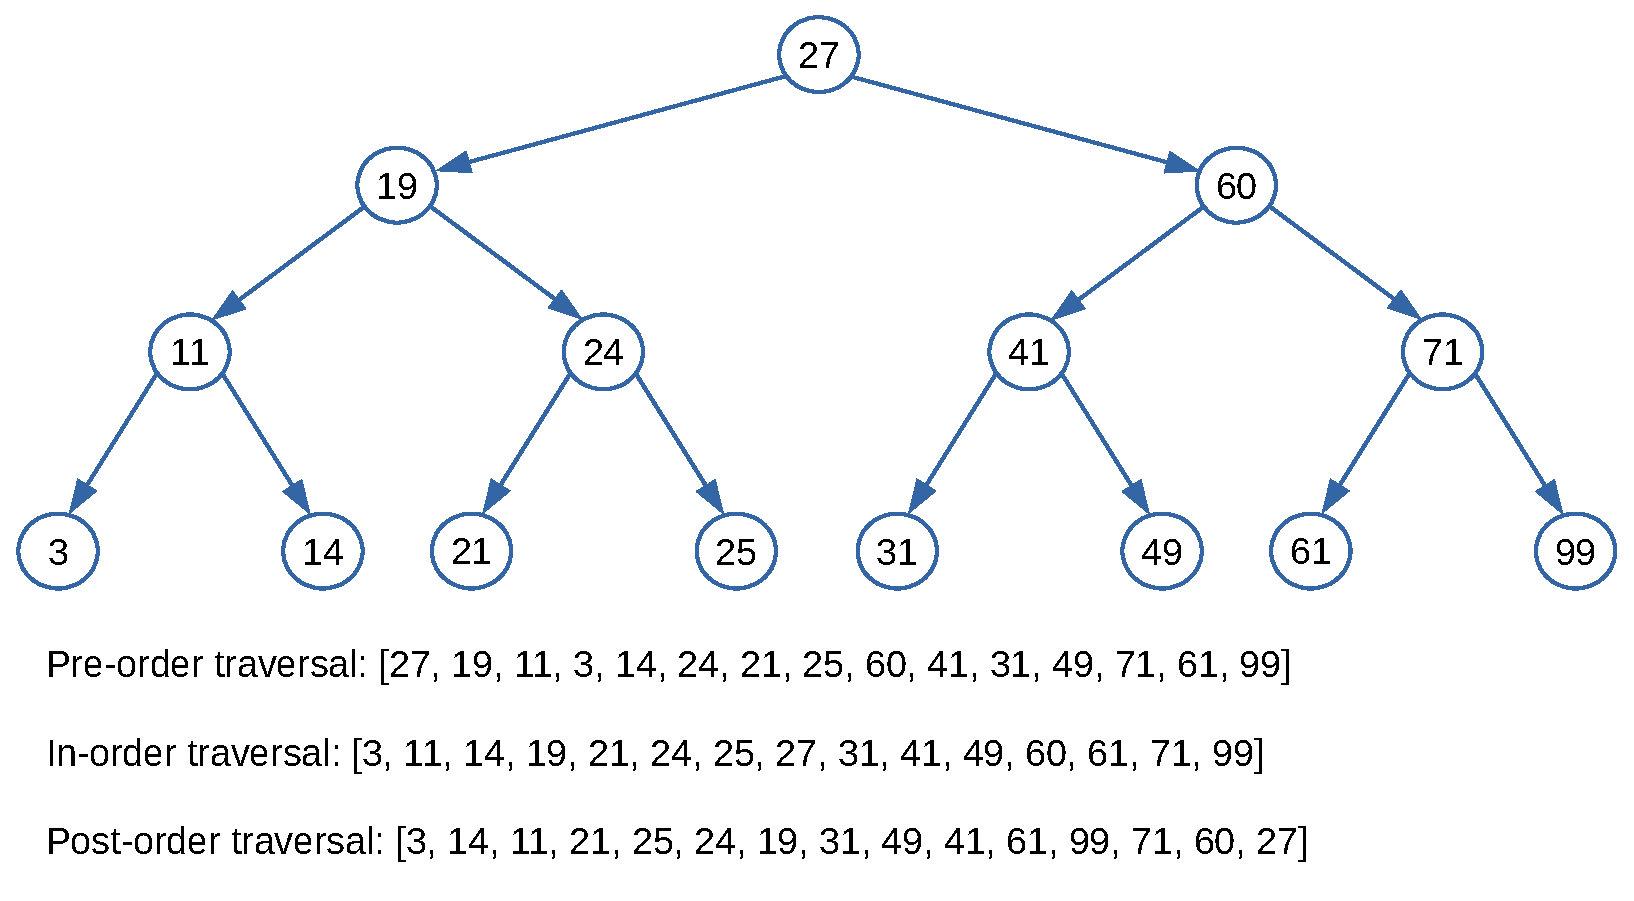
\includegraphics[scale=.6]{chapters/appendix/images/appendixtree/treesappendix_4.pdf}
		\caption[Breadth-first search example.]{Breadth-first search example.}
		\label{appendixtrees_3}
	\end{center}
\end{figure}

\begin{figure}[H]
\centering
\begin{tikzpicture}[every node/.style={circle,draw}, node distance=15mm, thick]

\node (na){$a$}
   child{node (nb) {$b$}
             child {node (nd) {$d$}}
             child {node (ne) {$e$}}
        }
   child{node (nc) {$c$}
			child[missing]
			child{node (nf) {$f$}}
		};
\draw ($(na) + (-2.3, 0.4)$) node[rectangle] {Breadth-first search};
\draw node[draw=none, rectangle, below=1mm of nd] {a, b, c, d, e, f};

\draw[->, >=stealth, ForestGreen] (na.west) -- (nb.north west);
\draw[->, >=stealth, ForestGreen] (nb.east) -- (nc.west);
\draw[->, >=stealth, ForestGreen] (nc.west) -- (nd.north east);
\draw[->, >=stealth, ForestGreen] (nd.east) -- (ne.west);
\draw[->, >=stealth, ForestGreen] (ne.east) -- (nf.west);

% Queue 1
\draw ($(na) + (3, 0.4)$) node[draw=none, rectangle, align=left] (queue) {Queue};

\draw[-] ($(queue.west) + (0,-4mm)$) -- ($(queue.west) + (0,-20mm)$);
\draw[-] ($(queue.west) + (10mm,-4mm)$) -- ($(queue.west) + (10mm,-20mm)$);
\draw ($(queue.south) + (-2.5mm,-13.5mm)$) node[draw, rectangle, rounded corners, minimum width=0.5cm, minimum height=0.5cm] (a1) {a};
\draw ($(queue.south) + (0,-22mm)$) node[draw, rectangle, minimum width=0.6cm, minimum height=0.6cm] (visited) {\textcolor{ForestGreen}{a}};
\path[->, >=stealth] ($(a1.north west) + (-10mm,3mm)$) edge [bend left=20] node[draw=none, xshift=-6pt, yshift=-7pt] {enq} (a1.north west);
\path[->, >=stealth] (a1.south west) edge [bend left=20] node[draw=none, xshift=-6pt, yshift=7pt] {deq} ($(a1.north east) + (-15mm, -10mm)$);

% queue 2
\draw ($(queue) + (1, 0)$) node[draw=none, rectangle, align=left] (queue1) {};
\draw[-] ($(queue1.west) + (0,-4mm)$) -- ($(queue1.west) + (0,-20mm)$);
\draw[-] ($(queue1.west) + (10mm,-4mm)$) -- ($(queue1.west) + (10mm,-20mm)$);
\draw ($(queue1.south) + (3.5mm,-15mm)$) node[draw, rectangle, rounded corners, minimum width=0.5cm, minimum height=0.5cm] (b2) {d};
\draw ($(queue1.south) + (3.5mm,-9mm)$) node[draw, rectangle, rounded corners, minimum width=0.5cm, minimum height=0.5cm] (c2) {c};
\draw[->, >=stealth] (a1.east) -- (b2.west);
\draw[->, >=stealth] (a1.east) -- (c2.west);
\draw ($(visited.east) + (10mm,0)$) node[draw, rectangle, minimum width=0.6cm, minimum height=0.6cm] {\textcolor{ForestGreen}{a, b}};

% queue 3
\draw ($(queue1) + (1.5, 0)$) node[draw=none, rectangle, align=left] (queue2) {};
\draw[-] ($(queue2.west) + (0,-4mm)$) -- ($(queue2.west) + (0,-20mm)$);
\draw[-] ($(queue2.west) + (10mm,-4mm)$) -- ($(queue2.west) + (10mm,-20mm)$);
\draw ($(queue2.south) + (3.5mm,-15mm)$) node[draw, rectangle, rounded corners, minimum width=0.5cm, minimum height=0.5cm] (c3) {c};
\draw ($(queue2.south) + (3.5mm,-9mm)$) node[draw, rectangle, rounded corners, minimum width=0.5cm, minimum height=0.5cm] (d3) {d};
\draw ($(queue2.south) + (3.5mm,-3mm)$) node[draw, rectangle, rounded corners, minimum width=0.5cm, minimum height=0.5cm] (e3) {e};
\draw[->, >=stealth] (b2.east) -- (d3.west);
\draw[->, >=stealth] (b2.east) -- (e3.west);
\draw ($(visited.east) + (25mm,0)$) node[draw, rectangle, minimum width=0.6cm, minimum height=0.6cm] {\textcolor{ForestGreen}{a, b, c}};

% queue 4
\draw ($(queue2) + (1.5, 0)$) node[draw=none, rectangle, align=left] (queue3) {};
\draw[-] ($(queue3.west) + (0,-4mm)$) -- ($(queue3.west) + (0,-20mm)$);
\draw[-] ($(queue3.west) + (10mm,-4mm)$) -- ($(queue3.west) + (10mm,-20mm)$);
\draw ($(queue3.south) + (3.5mm,-15mm)$) node[draw, rectangle, rounded corners, minimum width=0.5cm, minimum height=0.5cm] (d4) {d};
\draw ($(queue3.south) + (3.5mm,-9mm)$) node[draw, rectangle, rounded corners, minimum width=0.5cm, minimum height=0.5cm] (e4) {e};
\draw ($(queue3.south) + (3.5mm,-3mm)$) node[draw, rectangle, rounded corners, minimum width=0.5cm, minimum height=0.5cm] (f4) {f};
\draw ($(visited.east) + (44mm,0)$) node[draw, rectangle, minimum width=0.6cm, minimum height=0.6cm] {\textcolor{ForestGreen}{a, b, c, d}};

% queue 5
\draw ($(queue) + (-0.45, -2.5)$) node[draw=none, rectangle, align=left] (queue4) {};
\draw[-] ($(queue4.west) + (0,-4mm)$) -- ($(queue4.west) + (0,-20mm)$);
\draw[-] ($(queue4.west) + (10mm,-4mm)$) -- ($(queue4.west) + (10mm,-20mm)$);
\draw ($(queue4.south) + (3.5mm,-15mm)$) node[draw, rectangle, rounded corners, minimum width=0.5cm, minimum height=0.5cm] (e5) {e};
\draw ($(queue4.south) + (3.5mm,-9mm)$) node[draw, rectangle, rounded corners, minimum width=0.5cm, minimum height=0.5cm] (f4) {f};
\draw ($(queue4.south) + (1mm,-23mm)$) node[draw, rectangle, minimum width=0.6cm, minimum height=0.6cm] {\textcolor{ForestGreen}{a, b, c, d, e}};

% queue 6
\draw ($(queue4) + (1.45, 0)$) node[draw=none, rectangle, align=left] (queue5) {};
\draw[-] ($(queue5.west) + (0,-4mm)$) -- ($(queue5.west) + (0,-20mm)$);
\draw[-] ($(queue5.west) + (10mm,-4mm)$) -- ($(queue5.west) + (10mm,-20mm)$);
\draw ($(queue5.south) + (3.5mm,-15mm)$) node[draw, rectangle, rounded corners, minimum width=0.5cm, minimum height=0.5cm] (f5) {f};
\draw ($(queue5.south) + (10mm,-23mm)$) node[draw, rectangle, minimum width=0.6cm, minimum height=0.6cm] {\textcolor{ForestGreen}{a, b, c, d, e, f}};

% queue 7
\draw ($(queue5) + (1.5, 0)$) node[draw=none, rectangle, align=left] (queue6) {};
\draw[-] ($(queue6.west) + (0,-4mm)$) -- ($(queue6.west) + (0,-20mm)$);
\draw[-] ($(queue6.west) + (10mm,-4mm)$) -- ($(queue6.west) + (10mm,-20mm)$);
\draw ($(queue6.east) + (20mm,-10mm)$) node[draw=none, rectangle, minimum width=0.6cm, minimum height=0.6cm] {\textcolor{BrickRed}{queue empty}};

\end{tikzpicture}

\caption[Breadth-first search example.]{Breadth-first search example.}
\label{appendixtrees_3}
\end{figure}

\section{Complexity Summary}